\documentclass[a4paper,oneside,11pt,article]{memoir}

% Check input
\usepackage[utf8]{inputenc}
\usepackage[T1]{fontenc}

% Fonts and microtype
\usepackage[danish,english]{babel}
\usepackage{lmodern}
\usepackage[final]{microtype}

\usepackage{url}
\usepackage{xspace}
\usepackage{amsmath}
\usepackage{graphicx}

\begin{document}
\chapter{Error function}
In mathematics, the error function (also called the Gauss error function) is a special function (non-elementary) of sigmoid shape that occurs in probability, statistics, and partial differential equations describing diffusion. It is defined as
\begin{align}
\text{erf}(x) &= \frac{1}{\sqrt{(\pi)}} \int_{-x}^{x} \exp(- t^2) \, \text{d}t \nonumber\\
&= \frac{2}{\sqrt{(\pi)}} \int_{0}^{x} \exp(- t^2) \, \text{d}t.
\end{align}
In statistics, for nonnegative values of $x$, the error function has the following interpretation: for a random variable $X$ that is normally distributed with mean $0$ and variance $1/2$, erf$(x)$ describes the probability of $X$ falling in the range $[-x, x]$.

\chapter{The name 'error function'}
The error function is used in measurement theory (using probability and statistics), and its use in other branches of mathematics is typically unrelated to the characterization of measurement errors.

In statistics, it is common to have a variable ${\displaystyle Y}$ and its unbiased estimator ${\displaystyle {\hat {Y}}}$. The error is then defined as ${\displaystyle \varepsilon ={\hat {Y}}-Y}$. This makes the error a normally distributed random variable with mean $0$ (because the estimator is unbiased) and some variance ${\displaystyle \sigma ^{2}}$; this is written as ${\textstyle \varepsilon \sim {\mathcal {N}}(0,\,\sigma ^{2})}$. For the case where ${\textstyle \sigma ^{2}={\frac {1}{2}}}$, i.e.\@ an unbiased error variable ${\textstyle \varepsilon \sim {\mathcal {N}}(0,\,{\frac {1}{2}})}$, erf$(x)$ describes the probability of the error $\varepsilon$ falling in the range $[-x, x]$; in other words, the probability that the absolute error is no greater than $x$. This is true for any random variable with distribution ${\textstyle {\mathcal {N}}(0,\,{\frac {1}{2}})}$; but the application to error variables is how the error function got its name.[citation needed]

The previous paragraph can be generalized to any variance: given a variable (such as an unbiased error variable) ${\textstyle \varepsilon \sim {\mathcal {N}}(0,\,\sigma ^{2})}$, evaluating the error function at ${\textstyle \operatorname {erf} \left({\frac {x}{\sigma }}\cdot {\frac {1}{\sqrt {2}}}\right)}$ describes the probability of $\varepsilon$ falling in the range $[-x, x]$.[3] This is used in statistics to predict behavior of any sample with respect to the population mean. This usage is similar to the Q-function, which in fact can be written in terms of the error function.

\begin{figure}
\centering
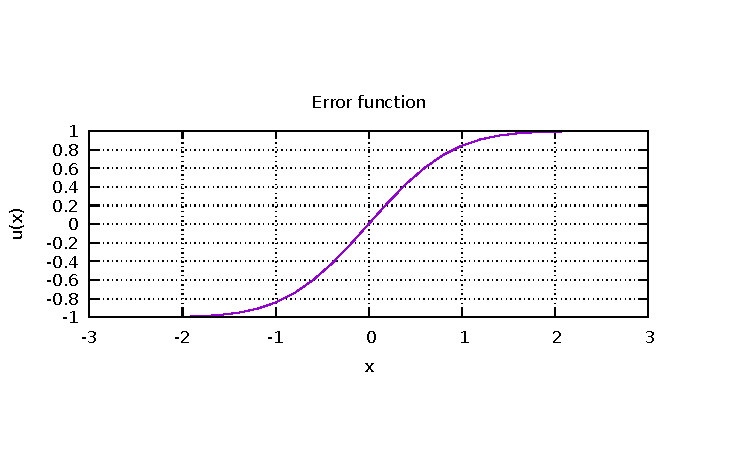
\includegraphics[width=1\linewidth]{plot}
\caption{Plot of error function erf$(x)$.}
\label{fig:plot}
\end{figure}

\end{document}
